\chapter{Methods}
\label{chp:methods}
% ---------------------------------------------------------------------------------------------------

% ===================================================================================================
\section{Simulation in hydrology}
% ===================================================================================================


% ---------------------------------------------------------------------------------------------------
\subsection{FullSWOF\_2D-v1.07.00}
% ---------------------------------------------------------------------------------------------------


% ===================================================================================================
\section{Emulation}
% ===================================================================================================


% ---------------------------------------------------------------------------------------------------
\subsection{Regression and interpolation methods}
% ---------------------------------------------------------------------------------------------------

\begin{itemize}
\itemsep0em
  \item explain the work done on regression and interpolation
  \item explain their relation with emulation
  \item explian extrapolation, when it can be done and how reliable it can be
\end{itemize}


% ===================================================================================================
\section{Development of \textit{FullSWOF\_2D} interaction tools}
% ===================================================================================================

\begin{itemize}
\itemsep0em
  \item explain the work done
  \item list the functions developed and their function
  \item mention \textit{fswof2d} repository
  \item explain how to install the package?? \noteseb{does this make sense here?? should go in the README}
\end{itemize}

As already mentioned in section \colseb{mention which section} \textit{FullSWOF\_2D-v1.07.00} was chosen as \emph{overland flow simulator} in order to generate the required datasets.
\textit{FullSWOF\_2D} needs at least three input files in order to run simulations:

\begin{itemize}
\itemsep0em
  \item \textit{topography}: a text file specifying the topography of the domain
  \item \textit{parameters}: a text file specifying the values set for the simulation parameters
  \item \textit{huv\_init}: a text file defining the initial conditions of the problem (initial water height and initial water velocity at every point of the grid)
\end{itemize}

In order to generate these files, interaction functions were developed with the open source tool \textit{Octave 4.2.1} \autocite{octave_community_gnu_2018}.
The interaction functions were grouped into the Octave package \textit{fswof2d} available at \url{https://bitbucket.org/binello7/fswof2d}.\\

The package includes the following functions, all of which are distributed under \textit {GPLv3} license \autocite{smith_quick_2014}.

\begin{itemize}
\itemsep0em
  \item center2node.m
  \item csec\_channel2lvlsym.m
  \item dataconvert.m
  \item extrude\_csec.m
  \item huv2file.m
  \item matplotlib\_cm.m
  \item node2center.m
  \item params2file.m
  \item read\_params.m
  \item topo2file.m
\end{itemize}

% ---------------------------------------------------------------------------------------------------
\subsection*{center2node.m}
% ---------------------------------------------------------------------------------------------------
\textit{function x = center2node (cx, x0)}\\




% ---------------------------------------------------------------------------------------------------
\subsection*{node2center.m}
% ---------------------------------------------------------------------------------------------------
\textit{function cx = node2center (x)}\\

\textit{FullSWOF\_2D} uses a regular uniform grid in order to solve the \emph{shallow water equation} with the finite volume method (FVM).
The equations are solved at the center of every cell.
After creating the vector defining the grid nodes, one can use the \textit{center2node} function to compute the centers of the grid cells.
This is particularly useful because the $(x,y)$ coordinates saved to the \textit{topography} file have to be the coordinates of the cell centers.
A short usage example would be:

\begin{lstlisting}
  # define the domain length in x-direction
  Lx = 100;
  # define the number of nodes
  Nx = 200;
  # create nodes of the regular grid in x-direction
  xn = linspace (0, Lx, Nx);
  # create vector of cell centers
  xc = node2cdenter (xn);
\end{lstlisting}



% ===================================================================================================
\section{Didactic example: emulator \noteseb{appropriate to use emulator here? other suggestions?} of " the weir equation"}
% ===================================================================================================

\begin{itemize}
\itemsep0em
  \item present it as a didactic example
  \item use it to compare GP (prior knowledge) with e.g. deep neural networks: how many points can we have?
  \item mention grid convergence study (results go in the appendix A)
  \item mention problem with FullSWOF boundary conditions
  \item define well results and methodology
\end{itemize}

% ---------------------------------------------------------------------------------------------------
\subsection{Methodology}
% ---------------------------------------------------------------------------------------------------

Short methodology of how the mechanistic emulator of the weir equation was developed, without subdivision into further subsections.


% ---------------------------------------------------------------------------------------------------
\subsection{Results and discussion}
% ---------------------------------------------------------------------------------------------------

Present and discuss briefly the results of this toy emulator.


% ===================================================================================================
\section{Generating the synthetic topography}
% ===================================================================================================







% ===================================================================================================
\section{Generating the datasets}
% ===================================================================================================




\begin{figure}[htpb]
  \centering
  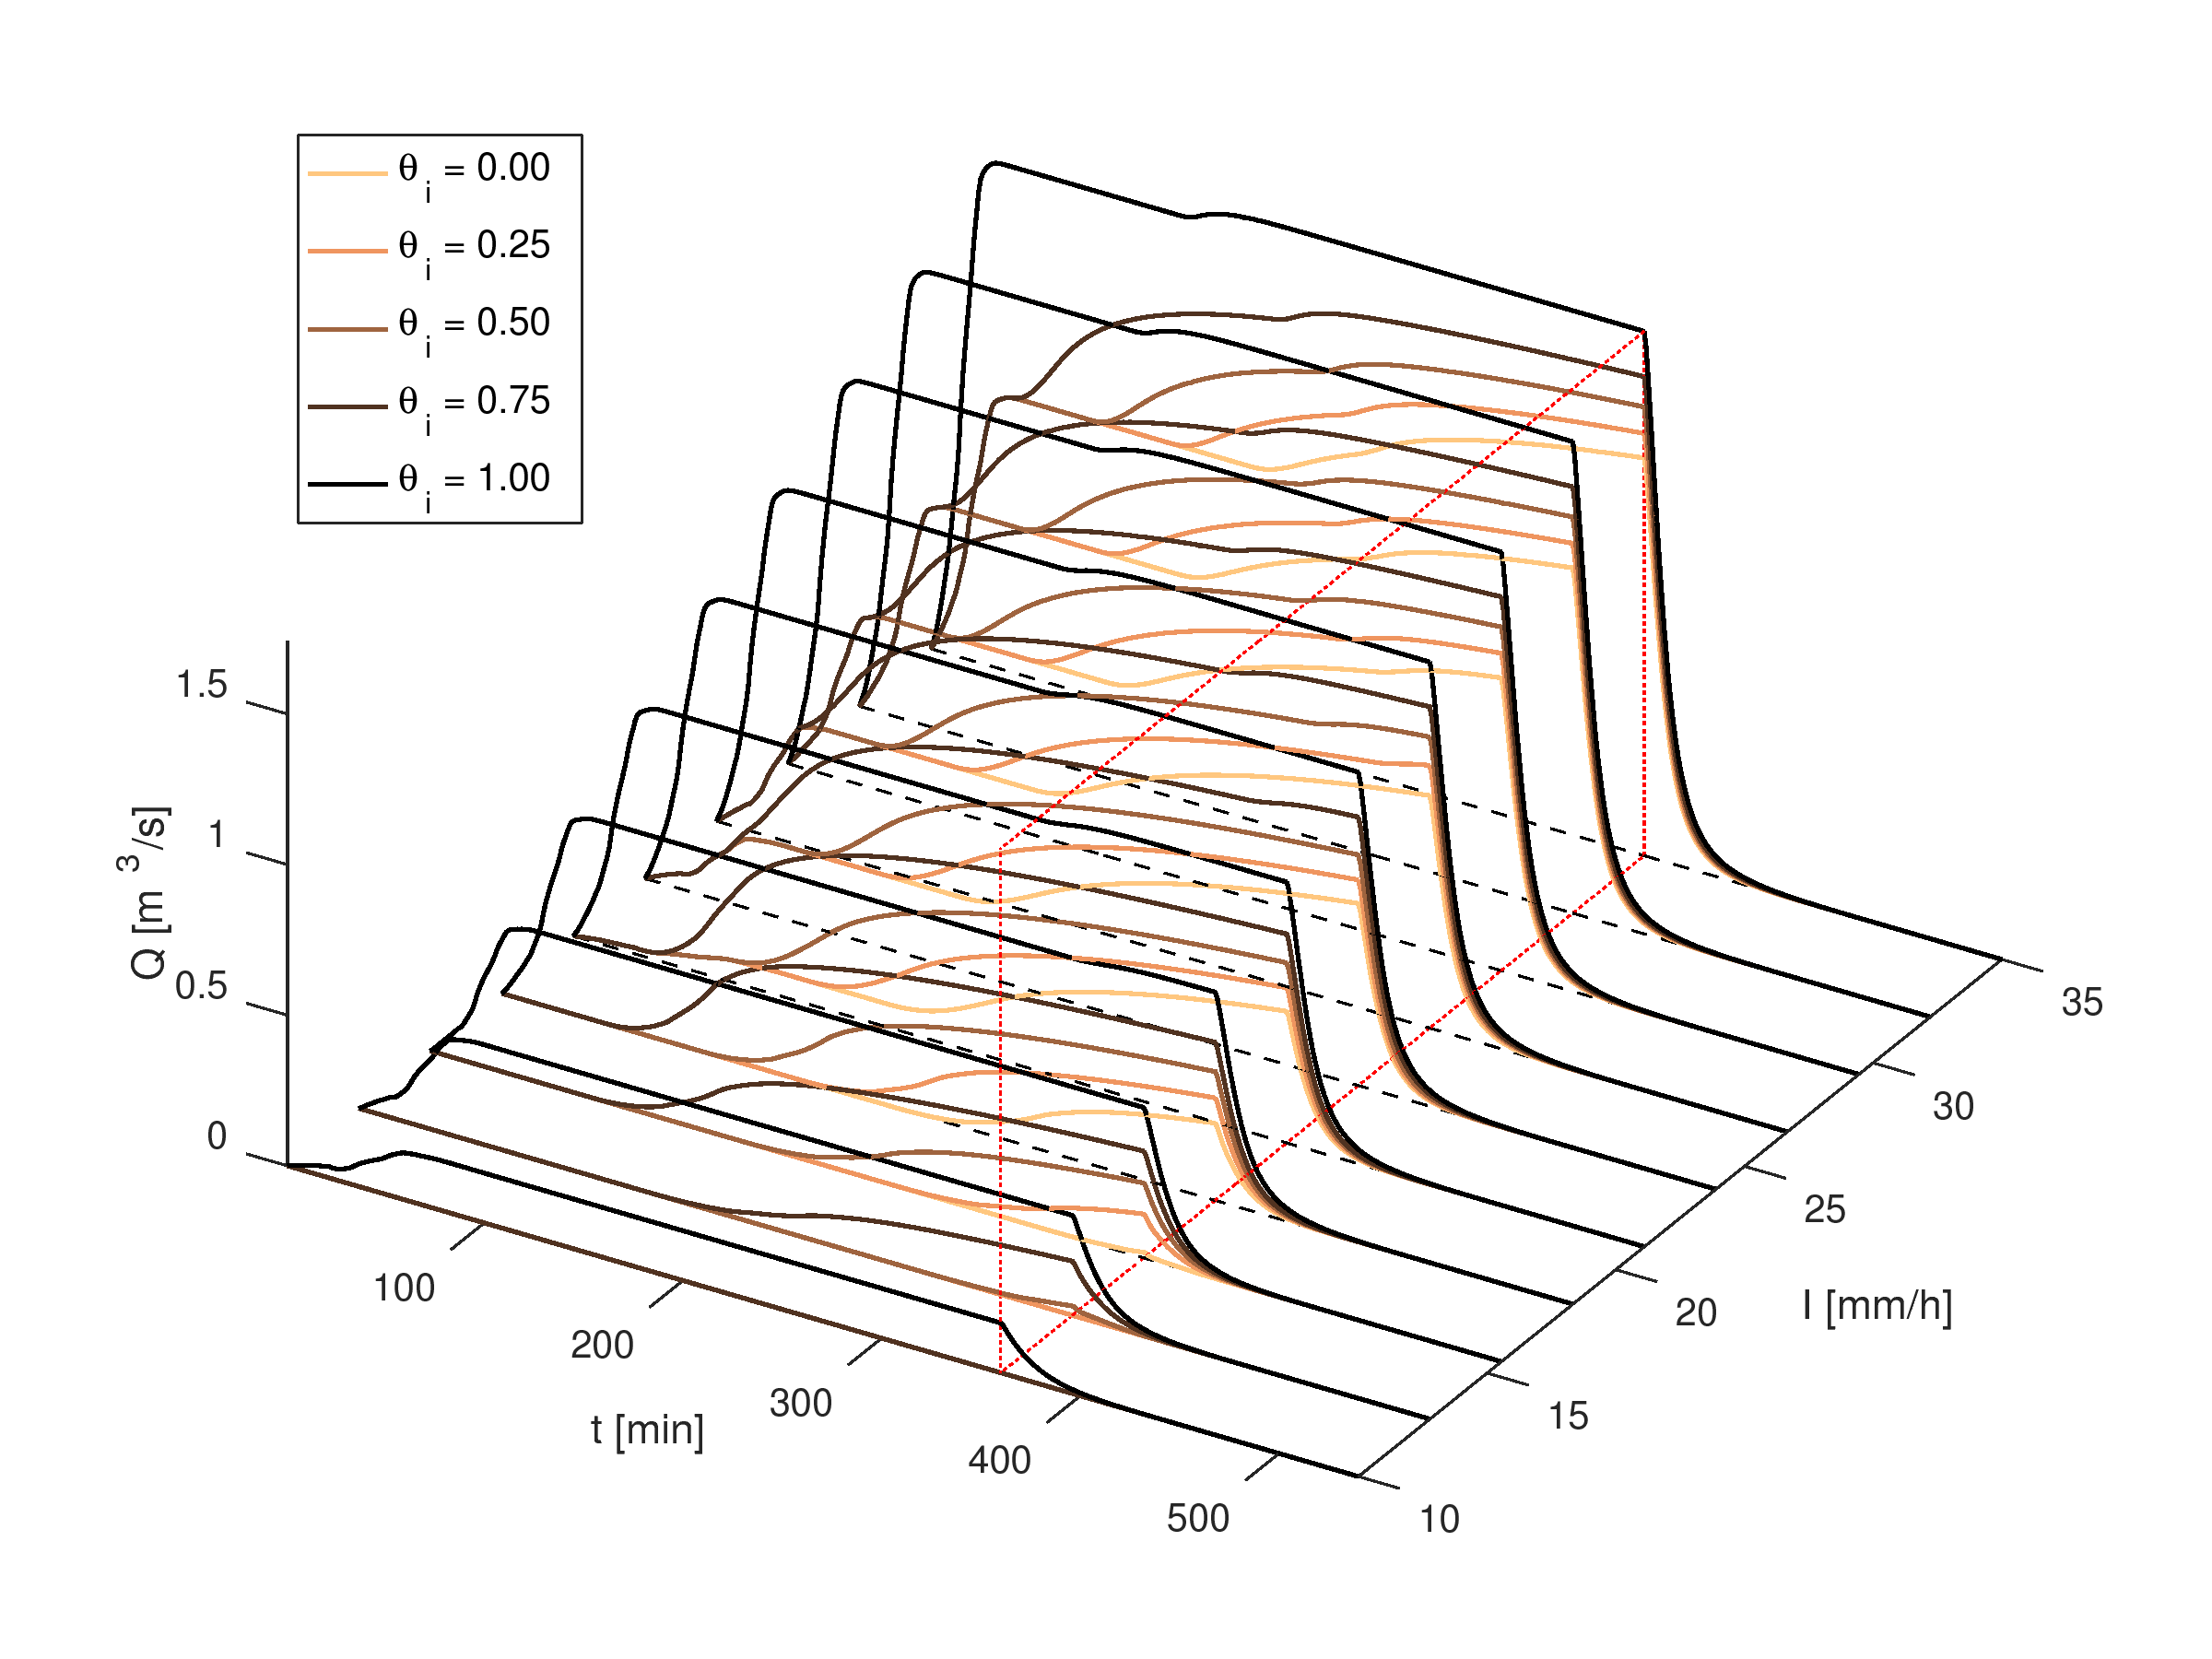
\includegraphics[width=0.75\textwidth]{Figures/hydrographs3d.png}
  \caption{Response hydrographs of the \num{50} simulations at the catchment outlet.}
  \label{fig:hydrographs3d}
\end{figure}


% ===================================================================================================
\section{Building the emulator}
% ===================================================================================================

% ---------------------------------------------------------------------------------------------------
\subsection{Classification emulator}
% ---------------------------------------------------------------------------------------------------

% ---------------------------------------------------------------------------------------------------
\subsection{Time-to-threshold emulator}
% ---------------------------------------------------------------------------------------------------


